%==============================================================================
% BLG 475E Software Quality and Testing - Term Project Report
% Authors: Ahmet Enes Çiğdem, Ali Eren Çiftçi, Taha Çali
%==============================================================================
\documentclass[12pt, a4paper]{article}

%--- Packages -----------------------------------------------------------------
\usepackage[utf8]{inputenc}
\usepackage[T1]{fontenc}
\usepackage[english]{babel}
\usepackage{geometry}
\usepackage{graphicx}
\usepackage{booktabs}
\usepackage{array}
\usepackage{tabularx}
\usepackage{longtable}
\usepackage{multirow}
\usepackage{caption}
\usepackage{subcaption}
\usepackage{amsmath}
\usepackage{amssymb}
\usepackage{hyperref}
\usepackage{listings}
\usepackage{xcolor}
\usepackage{float}
\usepackage{enumitem}
\usepackage{titlesec}
\usepackage{fancyhdr}
\usepackage{cite}
\usepackage{url}
\usepackage{pdflscape}
\usepackage{pgfplots}
\pgfplotsset{compat=1.18}

%--- Page Layout --------------------------------------------------------------
\geometry{
    top=2.5cm,
    bottom=2.5cm,
    left=2.5cm,
    right=2.5cm
}

%--- Header / Footer ----------------------------------------------------------
\pagestyle{fancy}
\fancyhf{}
\fancyhead[L]{\small BLG 475E -- Software Quality and Testing}
\fancyhead[R]{\small Term Project Report}
\fancyfoot[C]{\thepage}
\renewcommand{\headrulewidth}{0.4pt}
\renewcommand{\footrulewidth}{0pt}

%--- Code Listing Style -------------------------------------------------------
\definecolor{codebg}{RGB}{245,245,245}
\definecolor{codegreen}{RGB}{0,128,0}
\definecolor{codegray}{RGB}{128,128,128}
\definecolor{codeblue}{RGB}{0,0,200}
\definecolor{codepurple}{RGB}{128,0,128}

\lstdefinestyle{javastyle}{
    backgroundcolor=\color{codebg},
    basicstyle=\ttfamily\footnotesize,
    breaklines=true,
    captionpos=b,
    commentstyle=\color{codegreen}\itshape,
    keywordstyle=\color{codeblue}\bfseries,
    stringstyle=\color{codepurple},
    numberstyle=\tiny\color{codegray},
    numbers=left,
    numbersep=5pt,
    frame=single,
    rulecolor=\color{codegray},
    tabsize=4,
    language=Java,
    showstringspaces=false
}

\lstdefinestyle{pythonstyle}{
    backgroundcolor=\color{codebg},
    basicstyle=\ttfamily\footnotesize,
    breaklines=true,
    captionpos=b,
    commentstyle=\color{codegreen}\itshape,
    keywordstyle=\color{codeblue}\bfseries,
    stringstyle=\color{codepurple},
    numberstyle=\tiny\color{codegray},
    numbers=left,
    numbersep=5pt,
    frame=single,
    rulecolor=\color{codegray},
    tabsize=4,
    language=Python,
    showstringspaces=false
}

\lstset{style=javastyle}

%--- Hyperref Setup -----------------------------------------------------------
\hypersetup{
    colorlinks=true,
    linkcolor=blue!70!black,
    citecolor=green!50!black,
    urlcolor=blue!80!black
}

%--- Title Information --------------------------------------------------------
\title{
    \vspace{-1cm}
    \textbf{BLG 475E -- Software Quality and Testing} \\[0.5cm]
    \Large\textbf{Term Project Report:} \\
    \Large{LLM-Based Test Generation and Evaluation \\
    Using the HumanEval Dataset}
    \vspace{0.5cm}
}

\author{
    \textbf{Ahmet Enes \c{C}i\u{g}dem} \\ 150220079 \\[0.3cm]
    \textbf{Ali Eren \c{C}ift\c{c}i} \\ 150220022 \\[0.3cm]
    \textbf{Taha \c{C}ali} \\ 150220050
}

\date{\today}

%==============================================================================
\begin{document}

%--- Title Page ---------------------------------------------------------------
\maketitle
\thispagestyle{empty}

\begin{abstract}
% TODO: Write a concise abstract summarizing the project objectives, methodology,
% key findings, and conclusions. (150--250 words recommended)
\end{abstract}

\newpage
\tableofcontents
\newpage

%==============================================================================
% SECTION I: Introduction and Literature Review
%==============================================================================
\section{Introduction and Literature Review}
\label{sec:introduction}

\subsection{Introduction}
% TODO: Introduce the role of Large Language Models (LLMs) in code generation
% and software testing. Discuss why automated test generation is important
% and how LLMs are changing the landscape.

\subsection{Literature Review}
This section reviews five recent studies that investigate the use of LLMs in automated test generation and code quality assurance.

\subsubsection{ChatUniTest: A Framework for LLM-Based Test Generation}
Chen et al.~\cite{chatunitest} present \textit{ChatUniTest}, an automated unit test generation framework that addresses two key weaknesses of LLM-based tools: limited context windows and insufficient validation of generated tests. The framework introduces an \textit{adaptive focal context} mechanism that extracts only the relevant method, class properties, and dependencies via AST parsing, rather than feeding the entire source file to the model. Generated tests pass through a Generation-Validation-Repair cycle that includes syntactic, compilation, and runtime checks, with both rule-based and LLM-based repair strategies. In evaluation, ChatUniTest achieved 59.6\% line coverage, outperforming TestSpark (42.1\%) and EvoSuite (38.2\%). This paper is directly relevant to our project since our workflow similarly relies on iterative prompt construction and post-generation validation to obtain compilable and correct unit tests from LLMs.

\subsubsection{Mutation-Guided LLM-Based Test Generation at Meta}
Foster et al.~\cite{mutation_meta} describe Meta's \textit{Automated Compliance Hardening (ACH)} system, which combines mutation testing with LLM-based test generation. Rather than prompting an LLM to ``write tests'' generically, ACH first generates targeted mutants---simulated faults specific to a concern such as privacy---and then instructs the LLM to produce tests that kill these mutants. Deployed on 10,795 Kotlin classes across seven Meta platforms, ACH generated 571 hardening test cases with a 73\% developer acceptance rate. A notable finding is that 49\% of the valuable tests did not increase line coverage, demonstrating that coverage alone is an insufficient quality metric. This insight directly informs our manual assessment phase, where we complement coverage analysis with equivalence class partitioning and boundary testing.

\subsubsection{Adaptive Testing for LLM-Based Applications}
Yoon et al.~\cite{adaptive_testing} address the challenge of efficiently testing LLM-powered applications by adapting \textit{Adaptive Random Testing (ART)} to text-based prompt templates. Their approach iteratively selects the most diverse candidate input---measured via string distance metrics such as Levenshtein and Jaccard---and dynamically adjusts selection based on prior pass/fail outcomes. The technique discovers failures significantly faster than random sampling while requiring fewer costly API calls. For our project, this work provides a theoretical foundation for the input diversity strategies we apply when designing equivalence classes and selecting varied test inputs from the HumanEval dataset.

\subsubsection{LLM-Based Code Generation for Golang Compiler Testing}
Gu et al.~\cite{golang_compiler} investigate using LLMs as intelligent fuzzers for compiler testing. By fine-tuning an LLM on a carefully filtered Go codebase and guiding generation with a coverage-based seed scheduling strategy, the authors achieved 3.38\% compiler code coverage---nearly eight times higher than standard Go fuzzing (0.44\%). The generated code exhibited only 2.79\% syntax errors and effectively zero undefined behaviors. Although our project targets Java unit tests rather than compiler fuzzing, this paper demonstrates how constrained, seed-guided LLM generation can produce high-quality code artifacts, reinforcing the value of prompt engineering and structured generation strategies in our own pipeline.

\subsubsection{LLM-Based Test-Driven Interactive Code Generation}
Fakhoury et al.~\cite{ticoder} propose \textit{TiCoder}, an interactive workflow where the LLM first generates unit tests from a natural language prompt to formalize user intent, and then produces the implementation code constrained by those tests. In a user study with 15 programmers, participants using TiCoder were significantly more likely to correctly evaluate AI-generated code and reported lower cognitive load. At scale, the approach improved pass@1 accuracy by approximately 46\% within five interaction rounds. This paper is highly relevant to our project: it validates the test-driven philosophy we adopt in Phase~1, where LLM-generated tests serve as the specification against which code correctness is evaluated, and it motivates the iterative refinement approach we use in both our agentic and semi-agentic workflows.

%==============================================================================
% SECTION II: LLM Selection and Methodology
%==============================================================================
\section{LLM Selection and Methodology}
\label{sec:methodology}

\subsection{Selected LLMs}
For this project, we selected two distinct Large Language Models to generate solutions and test cases for the HumanEval dataset prompts. The selection was based on their state-of-the-art performance in code generation and reasoning tasks.

\begin{table}[H]
\centering
\caption{Comparison of Selected LLMs}
\label{tab:llm-comparison}
\begin{tabularx}{\textwidth}{l X X}
\toprule
\textbf{Criterion} & \textbf{LLM 1} & \textbf{LLM 2} \\
\midrule
Model Name       & Gemini Pro & Claude Opus 4.6 \\
Access Method    & Web Interface (Semi-Agentic) & Web Interface (Semi-Agentic) \\
Primary Role     & Code and test generation & Code and test generation \\
\bottomrule
\end{tabularx}
\end{table}

\subsection{Semi-Agentic Approach Justification}
Initially, we attempted to implement a fully automated agentic approach. We designed Python scripts to automate the prompting, code extraction, and test generation pipeline directly via the models' APIs. However, we encountered significant challenges regarding API rate limits and token exhaustion. The continuous stream of requests required for 30 HumanEval tasks, including generation, validation, and potential repair cycles, quickly depleted our free token quotas and incurred prohibitive costs.

To bypass these API constraints and complete the project successfully, we pivoted to a \textit{semi-agentic approach}. In this workflow, we manually managed the interaction with the LLMs through their respective web interfaces. We crafted the prompts locally, submitted them to the web UI, and manually extracted the generated code and tests to integrate them into our local Maven project.

\subsection{Advantages and Limitations}
The semi-agentic approach presented distinct advantages and limitations compared to a fully automated pipeline.

\textbf{Advantages:}
\begin{itemize}
    \item \textit{Cost Control:} By utilizing the web interfaces, we completely circumvented the API costs and token limits that stalled our initial automated approach.
    \item \textit{Enhanced Control and Observation:} Manually handling the prompts allowed us to closely monitor the models' reasoning processes in real-time, making it easier to adjust our prompt engineering strategies on the fly when models hallucinated or failed to follow instructions.
\end{itemize}

\textbf{Limitations:}
\begin{itemize}
    \item \textit{Increased Manual Effort:} The most significant drawback was the substantial manual labor required to copy, paste, format, and organize the code for 30 distinct tasks across two models.
    \item \textit{Reduced Scalability:} While effective for a subset of 30 prompts, this manual workflow is not scalable for evaluating the entire HumanEval dataset (164 tasks) or for integration into continuous integration/continuous deployment (CI/CD) pipelines.
\end{itemize}

%==============================================================================
% SECTION III: Phase 1 -- Unit Testing and Manual Assessment
%==============================================================================
\section{Phase 1: Unit Testing and Manual Assessment}
\label{sec:phase1}

\subsection{Prompt Selection Criteria}
% TODO: Explain your criteria for selecting the 30 specific prompts from
% the HumanEval dataset.

\subsection{Difficulty Categorization}
% TODO: Categorize the 30 prompts by difficulty (easy, moderate, hard).

\begin{table}[H]
\centering
\caption{HumanEval Prompt Categorization by Difficulty}
\label{tab:prompt-difficulty}
\begin{tabularx}{\textwidth}{l l X}
\toprule
\textbf{Difficulty} & \textbf{Task IDs} & \textbf{Description / Rationale} \\
\midrule
Easy     &  &  \\
Moderate &  &  \\
Hard     &  &  \\
\bottomrule
\end{tabularx}
\end{table}

\subsection{Base Testing Phase}
% TODO: Describe the base testing phase. Note any minor modifications made to
% expected values without altering the LLM-generated code.

\subsection{Manual Assessment Results}
% TODO: Present manual assessment results in tables, detailing equivalence class
% partitioning (valid and invalid classes) alongside boundary conditions.

% Template table for a single task's equivalence class analysis:
\begin{table}[H]
\centering
\caption{Equivalence Class Partitioning -- Task \#X}
\label{tab:ecp-taskX}
\begin{tabularx}{\textwidth}{l l X l}
\toprule
\textbf{Class ID} & \textbf{Type} & \textbf{Description} & \textbf{Expected Output} \\
\midrule
EC1 & Valid   &  &  \\
EC2 & Valid   &  &  \\
EC3 & Invalid &  &  \\
EC4 & Invalid &  &  \\
\midrule
\multicolumn{4}{l}{\textit{Boundary Conditions}} \\
\midrule
BC1 &  &  &  \\
BC2 &  &  &  \\
\bottomrule
\end{tabularx}
\end{table}

\subsection{Test Smell and Branch Coverage Analysis}
% TODO: Detail the test smell and branch coverage analysis utilized to
% improve your base tests.

\begin{table}[H]
\centering
\caption{Test Smell Analysis Summary}
\label{tab:test-smells}
\begin{tabularx}{\textwidth}{l l X l}
\toprule
\textbf{Task} & \textbf{Smell Type} & \textbf{Description} & \textbf{Action Taken} \\
\midrule
 &  &  &  \\
\bottomrule
\end{tabularx}
\end{table}

\begin{table}[H]
\centering
\caption{Branch Coverage Summary}
\label{tab:branch-coverage}
\begin{tabularx}{\textwidth}{l c c c}
\toprule
\textbf{Task} & \textbf{Base Coverage (\%)} & \textbf{Improved Coverage (\%)} & \textbf{Improvement} \\
\midrule
 &  &  &  \\
\bottomrule
\end{tabularx}
\end{table}

\subsection{Coverage Discussion and Input Mutations}
% TODO: Explain to what extent your tests cover the identified classes.
% Discuss any input mutations generated to address test failures.

%==============================================================================
% SECTION IV: Phase 2 -- Integration Testing
%==============================================================================
\section{Phase 2: Integration Testing}
\label{sec:phase2}

\subsection{BookScan Class Design}
% TODO: Outline the design of the BookScan Java class generated by the agents.

\begin{figure}[H]
\centering
% \includegraphics[width=0.8\textwidth]{images/bookscan_uml.png}
\caption{BookScan Class UML Diagram}
\label{fig:bookscan-uml}
\end{figure}

\subsection{Task Integration Details}
% TODO: Detail how the three tasks were integrated into the BookScan class.

\subsubsection{Task \#18 -- Substring}
% TODO: Describe the integration of the substring task.

\subsubsection{Task \#23 -- String Length}
% TODO: Describe the integration of the string length task.

\subsubsection{Task \#27 -- Upper-Lower Case}
% TODO: Describe the integration of the upper-lower case task.

\subsection{Integration Tests}
% TODO: Discuss the integration tests generated by the LLM agents and
% assess their effectiveness.

\begin{table}[H]
\centering
\caption{Integration Test Results Summary}
\label{tab:integration-results}
\begin{tabularx}{\textwidth}{l c c X}
\toprule
\textbf{Test Scenario} & \textbf{LLM 1} & \textbf{LLM 2} & \textbf{Notes} \\
\midrule
 & Pass/Fail & Pass/Fail &  \\
\bottomrule
\end{tabularx}
\end{table}

\subsection{Complex Integration Evaluation}
% TODO: Evaluate the model's performance in complex class integration scenarios.
% Detail any specific problems that occurred.

\subsection{Prompt Engineering: Unmodified vs.\ Edited Prompts}
% TODO: Compare the output generated using unmodified/combined prompts versus
% edited/combined prompts. Explain your prompt engineering approach.

\begin{table}[H]
\centering
\caption{Prompt Engineering Comparison}
\label{tab:prompt-engineering}
\begin{tabularx}{\textwidth}{l c c X}
\toprule
\textbf{Metric} & \textbf{Unmodified} & \textbf{Edited} & \textbf{Observation} \\
\midrule
Code Correctness    &  &  &  \\
Test Pass Rate      &  &  &  \\
Coverage            &  &  &  \\
Code Quality        &  &  &  \\
\bottomrule
\end{tabularx}
\end{table}

%==============================================================================
% SECTION V: Results, Analysis, and Refactoring
%==============================================================================
\section{Results, Analysis, and Refactoring}
\label{sec:results}

\subsection{Test Case Results}
% TODO: Provide clear tables or graphs visualizing the percentages of successful
% and failed test cases, alongside code correctness and error rates.

\begin{table}[H]
\centering
\caption{Overall Test Results by LLM}
\label{tab:overall-results}
\begin{tabularx}{\textwidth}{l c c c c}
\toprule
\textbf{Metric} & \textbf{LLM 1 (Unit)} & \textbf{LLM 1 (Integ.)} & \textbf{LLM 2 (Unit)} & \textbf{LLM 2 (Integ.)} \\
\midrule
Total Tests         &  &  &  &  \\
Passed              &  &  &  &  \\
Failed              &  &  &  &  \\
Pass Rate (\%)      &  &  &  &  \\
Code Correctness    &  &  &  &  \\
\bottomrule
\end{tabularx}
\end{table}

% Example: Bar chart for pass/fail visualization
\begin{figure}[H]
\centering
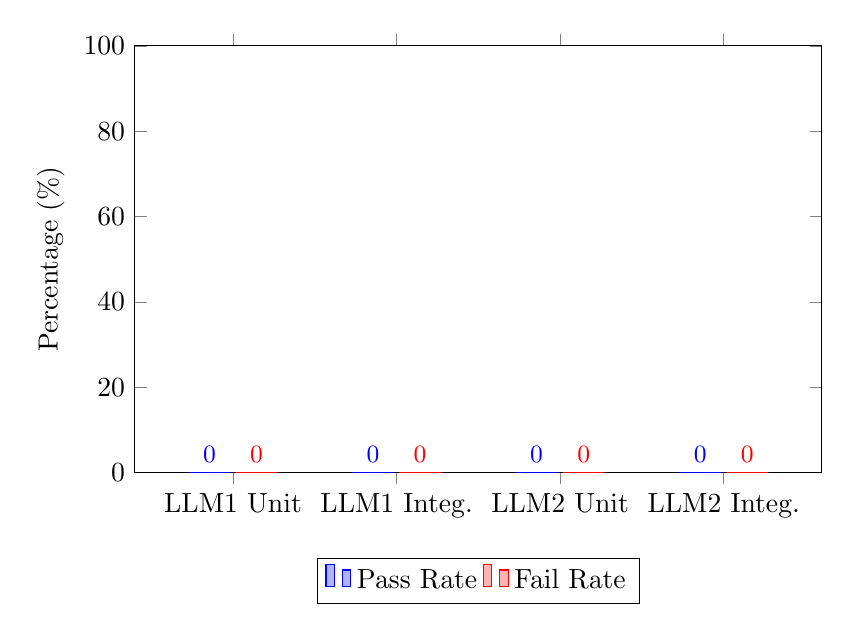
\begin{tikzpicture}
\begin{axis}[
    ybar,
    bar width=15pt,
    width=0.85\textwidth,
    height=7cm,
    ylabel={Percentage (\%)},
    symbolic x coords={LLM1 Unit, LLM1 Integ., LLM2 Unit, LLM2 Integ.},
    xtick=data,
    ymin=0, ymax=100,
    legend style={at={(0.5,-0.20)}, anchor=north, legend columns=2},
    nodes near coords,
    every node near coord/.append style={font=\small},
    enlarge x limits=0.2,
]
% TODO: Replace 0 values with actual data
\addplot coordinates {(LLM1 Unit,0) (LLM1 Integ.,0) (LLM2 Unit,0) (LLM2 Integ.,0)};
\addplot coordinates {(LLM1 Unit,0) (LLM1 Integ.,0) (LLM2 Unit,0) (LLM2 Integ.,0)};
\legend{Pass Rate, Fail Rate}
\end{axis}
\end{tikzpicture}
\caption{Test Pass/Fail Rates by LLM and Test Type}
\label{fig:pass-fail-chart}
\end{figure}

\subsection{Statistical Evaluation}
% TODO: Provide a statistical evaluation of the agents' performance
% and success rates.

\subsection{LLM Comparison}
% TODO: Include a comparison table for each LLM detailing metrics such as
% coverage and test cases per method.

\begin{table}[H]
\centering
\caption{Per-Method Comparison Between LLMs}
\label{tab:per-method-comparison}
\begin{tabularx}{\textwidth}{l c c c c}
\toprule
\textbf{Task} & \textbf{LLM 1 Coverage (\%)} & \textbf{LLM 1 Tests} & \textbf{LLM 2 Coverage (\%)} & \textbf{LLM 2 Tests} \\
\midrule
 &  &  &  &  \\
\bottomrule
\end{tabularx}
\end{table}

\subsection{Refactoring Process}
% TODO: Discuss the refactoring process. Detail how you guided the agent to
% make code corrections when tests failed during white-box or black-box testing.

\subsection{Agent-Generated Code Errors}
% TODO: Report on specific errors found in the agent-generated code.

\begin{table}[H]
\centering
\caption{Common Errors in Agent-Generated Code}
\label{tab:code-errors}
\begin{tabularx}{\textwidth}{l l X l}
\toprule
\textbf{Task} & \textbf{Error Type} & \textbf{Description} & \textbf{Resolution} \\
\midrule
 &  &  &  \\
\bottomrule
\end{tabularx}
\end{table}

%==============================================================================
% SECTION VI: Conclusion
%==============================================================================
\section{Conclusion}
\label{sec:conclusion}

% TODO: Summarize the capabilities and shortcomings of the chosen LLMs
% in both unit and integration testing pipelines.

%==============================================================================
% SECTION VII: Acknowledgments
%==============================================================================
\section{Acknowledgments}
\label{sec:acknowledgments}

\subsection{GitHub Repository}
% TODO: Provide the direct URL to your project's GitHub repository.
The source code and all artifacts for this project are available at:
\begin{center}
    \url{https://github.com/YOUR_REPO_URL_HERE}
\end{center}

\subsection{Work Distribution}
% TODO: Provide a detailed breakdown of the work distribution and
% specific duties among your 3-person group.

\begin{table}[H]
\centering
\caption{Work Distribution Among Team Members}
\label{tab:work-distribution}
\begin{tabularx}{\textwidth}{l l X}
\toprule
\textbf{Member} & \textbf{Student ID} & \textbf{Responsibilities} \\
\midrule
Ahmet Enes \c{C}i\u{g}dem & 150220079 &
% TODO: List specific duties
\\[0.5cm]
Ali Eren \c{C}ift\c{c}i & 150220022 &
% TODO: List specific duties
\\[0.5cm]
Taha \c{C}ali & 150220050 &
% TODO: List specific duties
\\
\bottomrule
\end{tabularx}
\end{table}

%==============================================================================
% SECTION VIII: References
%==============================================================================
% IEEE-style references
\bibliographystyle{IEEEtran}
% TODO: Create a references.bib file and uncomment the line below
% \bibliography{references}

% Alternatively, use manual references:
\begin{thebibliography}{99}

\bibitem{chatunitest}
Y.~Chen, Z.~Hu, C.~Zhi, J.~Han, S.~Deng, and J.~Yin,
``ChatUniTest: A framework for LLM-based test generation,''
in \textit{Companion Proc.\ 32nd ACM Int.\ Conf.\ Foundations of Software Engineering (FSE Companion '24)},
Porto de Galinhas, Brazil, Jul.\ 2024, pp.\ 572--576.
\url{https://doi.org/10.1145/3663529.3663801}

\bibitem{mutation_meta}
C.~Foster, A.~Gulati, M.~Harman, I.~Harper, K.~Mao, J.~Ritchey, H.~Robert, and S.~Sengupta,
``Mutation-guided LLM-based test generation at Meta,''
in \textit{33rd ACM Int.\ Conf.\ Foundations of Software Engineering (FSE Companion '25)},
Trondheim, Norway, Jun.\ 2025.
\url{https://doi.org/10.1145/3696630.3728544}

\bibitem{adaptive_testing}
J.~Yoon, R.~Feldt, and S.~Yoo,
``Adaptive testing for LLM-based applications: A diversity-based approach,''
in \textit{Proc.\ IEEE/ACM Int.\ Conf.\ Software Engineering (ICSE '25)},
2025.

\bibitem{golang_compiler}
Q.~Gu \textit{et al.},
``LLM-based code generation method for Golang compiler testing,''
in \textit{Proc.\ 31st ACM Joint European Software Engineering Conf.\ and Symp.\ on the Foundations of Software Engineering (ESEC/FSE '23)},
San Francisco, CA, USA, Dec.\ 2023.

\bibitem{ticoder}
S.~Fakhoury, A.~Naik, G.~Sakkas, S.~Chakraborty, and S.~K.~Lahiri,
``LLM-based test-driven interactive code generation: User study and empirical evaluation,''
\textit{IEEE Trans.\ Softw.\ Eng.}, vol.~50, no.~9, pp.\ 2254--2267, Sep.\ 2024.
\url{https://doi.org/10.1109/TSE.2024.3428972}

\bibitem{humaneval}
M.~Chen \textit{et al.},
``Evaluating large language models trained on code,''
\textit{arXiv preprint arXiv:2107.03374}, 2021.

\end{thebibliography}

%==============================================================================
\end{document}
